% =====================================================================
%  FacultyConnect: An Academic Collaboration Hub  --  Detailed Report
%  Format : IEEE conference (IEEEtran), same as the earlier 2-page report
%  Overleaf: New Project -> Upload Project -> select this .zip
%            Menu -> Compiler: pdfLaTeX
% =====================================================================
\documentclass[conference]{IEEEtran}
\IEEEoverridecommandlockouts

\usepackage{cite}
\usepackage{amsmath,amssymb,amsfonts}
\usepackage{algorithm}
\usepackage{algpseudocode}
\usepackage{graphicx}
\usepackage{textcomp}
\usepackage{xcolor}
\usepackage{booktabs}
\usepackage{tabularx}
\usepackage{array}
\usepackage{multirow}
\usepackage{enumitem}
\usepackage{tikz}
\usetikzlibrary{positioning,arrows.meta,shapes.geometric,shapes.multipart,fit,backgrounds,calc}
\usepackage{pgfgantt}
\usepackage{listings}
\usepackage[hidelinks]{hyperref}
\usepackage{url}

\definecolor{brand}{HTML}{5A4AD1}
\definecolor{coral}{HTML}{D9533D}
\definecolor{mint}{HTML}{1F9E74}
\definecolor{codebg}{HTML}{F6F5FB}
\setlist{nosep,leftmargin=1.2em}
\newcolumntype{Y}{>{\raggedright\arraybackslash}X}

\lstset{basicstyle=\ttfamily\scriptsize,backgroundcolor=\color{codebg},frame=single,
  rulecolor=\color{brand!40},breaklines=true,columns=fullflexible,xleftmargin=2pt,xrightmargin=2pt}

\tikzset{
  box/.style={draw=brand,rounded corners=2pt,fill=brand!6,align=center,font=\scriptsize,inner sep=3pt,minimum height=6.5mm},
  ext/.style={draw=coral,rounded corners=2pt,fill=coral!7,align=center,font=\scriptsize,inner sep=3pt,minimum height=6.5mm},
  store/.style={draw=mint,fill=mint!7,align=center,font=\scriptsize,inner sep=3pt,minimum height=6mm},
  arr/.style={-{Latex[length=1.6mm]},semithick,draw=black!65},
  lbl/.style={font=\tiny,fill=white,inner sep=1pt}
}

\begin{document}

\title{FacultyConnect: An Academic Collaboration Hub}

\author{
\IEEEauthorblockN{Vani Tripathi}
\IEEEauthorblockA{Roll No. 1024160073\\
vtripathi\_be24@thapar.edu}
\and
\IEEEauthorblockN{Agrim Mittal}
\IEEEauthorblockA{Roll No. 1024160068\\
Amittal3\_be24@thapar.edu}
\and
\IEEEauthorblockN{Shriyam Bhardwaj}
\IEEEauthorblockA{Roll No. 1024160062\\
sbhardwaj1\_be24@thapar.edu}
}

\maketitle

% =====================================================================
\begin{abstract}
FacultyConnect is a centralized academic collaboration platform that connects students with suitable faculty members for academic projects, research, coursework and guidance. At most institutes, information about faculty expertise, research interests, current projects, course material and availability is spread across department web pages, notice boards, e-mail threads and messaging groups, so students spend considerable time simply finding the right person and the right resource. FacultyConnect addresses this through a searchable faculty directory, rich faculty profiles, a single date-wise \emph{All work} timeline of everything a faculty member has shared, assignments with progress tracking, an interactive question bank, structured student--faculty messaging, and an AI-assisted faculty recommendation engine with a deterministic keyword-overlap fallback. The system defines Student, Faculty and Administrator roles. This report presents the complete software engineering life cycle of the project: requirement analysis and specification, system design (architecture, data-flow, entity--relationship, use-case and sequence models), implementation of a working prototype deployed on Vercel, the recommendation and timeline algorithms, a test plan with twelve executed test cases, feasibility and project-management analysis, and directions for future work. The prototype satisfies all core functional requirements, loads as a single lightweight page, works on mobile screens, and degrades gracefully when network services are unavailable.
\end{abstract}

\begin{IEEEkeywords}
FacultyConnect, academic collaboration, faculty discovery, recommendation system, timeline interface, single-page application, software engineering
\end{IEEEkeywords}

% =====================================================================
\section{Introduction}

Students require faculty guidance for academic projects, final-year capstones, summer research, technical doubts, competitions and career decisions. Thapar Institute of Engineering and Technology (TIET), like most large engineering institutes, has many departments and hundreds of faculty members, each with distinct research interests, ongoing projects and courses. However, information about who works on what, which projects are open, and what material has been shared is typically scattered across department web pages that are updated infrequently, personal pages, learning-management courses, e-mail and informal messaging groups.

This fragmentation affects both sides. A student interested in, say, automated code review has no straightforward way to discover that a particular assistant professor runs a group on exactly that topic. A student looking for last semester's mid-semester test (MST) solutions must search through several chat groups. Faculty members, in turn, re-share the same files in multiple places, have no structured channel to advertise openings, and receive unstructured requests over personal e-mail that are hard to track.

FacultyConnect is proposed as a centralized academic collaboration hub that brings students, faculty, resources and opportunities together on a single platform. The platform is role-aware: students discover and interact, faculty publish and respond, and administrators govern data quality.

\subsection{Motivation}
Three observations motivated the project. First, \emph{discovery} is the bottleneck: once a student finds the right faculty member, collaboration usually follows, but finding that person is slow and depends on word of mouth. Second, \emph{shared material lacks context}: files circulated over messaging apps lose their date, course and author, so students cannot tell what is current. Third, \emph{communication is unstructured}: requests arrive without a stated purpose, which makes them easy to overlook.

\subsection{Contributions}
The main contributions of this work are:
\begin{enumerate}
  \item A requirements specification for a student--faculty collaboration platform covering three user roles, twelve functional and six non-functional requirements.
  \item A layered system design with data-flow, entity--relationship, use-case and sequence models.
  \item A unified, chronologically grouped \emph{All work} timeline that merges uploads, assignments, lecture units and question-bank additions into one view, replacing separate upload lists.
  \item A lightweight faculty recommendation method based on keyword overlap with research-area descriptions, optionally upgraded by a language model.
  \item A working, publicly deployed prototype and a documented test campaign.
\end{enumerate}

\subsection{Organization of the Report}
Section~II reviews existing approaches. Section~III states the problem and objectives. Section~IV gives the software requirements specification. Section~V describes the proposed system and Section~VI its design. Section~VII covers implementation and algorithms, Section~VIII the prototype interface, and Section~IX testing. Sections~X--XII discuss results, feasibility and project management, and Sections~XIII--XIV conclude with limitations, future scope and conclusions.

% =====================================================================
\section{Literature Review and Existing Systems}

\subsection{Institutional Web Pages}
Most universities publish faculty lists on department websites. These pages typically provide name, designation, qualifications and a short list of interests. They are static, are maintained centrally by a web team, and rarely include current projects, openings or course material. They are also not searchable across departments by research topic.

\subsection{Learning Management Systems}
Platforms such as Moodle and Google Classroom organize course content, assignments and announcements per course \cite{moodle,classroom}. They work well once a student is enrolled in a course, but they are course-centric rather than faculty-centric: a student cannot browse a faculty member's research, discover openings outside enrolled courses, or find which faculty member best matches a project idea.

\subsection{Researcher Profile Databases}
National and international researcher directories such as INFLIBNET's Vidwan expert database and IRINS institutional repositories, as well as academic networks such as Google Scholar and ResearchGate, list publications and expertise \cite{vidwan,irins,scholar}. They are rich in publication data but are oriented towards researchers and funding bodies; they do not provide course resources, assignments, question banks or structured student requests.

\subsection{Recommendation Approaches}
Expert-finding and recommender systems commonly use content-based filtering, where items (here, faculty) are described by text features and matched against a user query \cite{ricci,balog}. Simple term-overlap or TF--IDF scoring is transparent and needs no training data, while embedding-based semantic matching captures synonyms at the cost of a model dependency \cite{reimers}. FacultyConnect adopts term overlap for its baseline because it is explainable to students and feasible within a semester, with semantic matching as an optional enhancement.

\subsection{Gap Identified}
Table~\ref{tab:compare} summarizes the comparison. No single existing system combines faculty discovery by research interest, faculty-centric shared resources with dates, opportunities, and structured communication. FacultyConnect targets this gap.

\begin{table}[t]
\caption{Comparison with Existing Approaches}
\label{tab:compare}
\centering\scriptsize
\setlength{\tabcolsep}{3pt}
\begin{tabular}{@{}lccccc@{}}
\toprule
\textbf{Capability} & \textbf{Dept.} & \textbf{LMS} & \textbf{Researcher} & \textbf{Chat} & \textbf{Faculty-}\\
 & \textbf{site} &  & \textbf{DB} & \textbf{groups} & \textbf{Connect}\\
\midrule
Search by research area   & -- & -- & \checkmark & -- & \checkmark\\
Faculty-centric resources & -- & partial & -- & partial & \checkmark\\
Dated, ordered material   & -- & \checkmark & -- & -- & \checkmark\\
Assignments \& progress   & -- & \checkmark & -- & -- & \checkmark\\
Question bank / practice  & -- & partial & -- & -- & \checkmark\\
Structured requests       & -- & -- & -- & -- & \checkmark\\
Faculty recommendation    & -- & -- & partial & -- & \checkmark\\
\bottomrule
\end{tabular}
\end{table}

% =====================================================================
\section{Problem Statement and Objectives}

\subsection{Problem Statement}
The main problem is the absence of a centralized mechanism through which students can discover suitable faculty based on their interests, skills, research areas and project requirements, and access everything those faculty have shared in an organized, dated form. Faculty members also need an organized method to publish material and opportunities and to handle student requests.

\subsection{Objectives}
\begin{enumerate}
  \item Help students find suitable faculty quickly through search, filters and recommendations.
  \item Centralize academic resources, with each faculty member's material available in one chronological timeline.
  \item Promote research and project collaboration by making openings visible.
  \item Provide structured student--faculty communication with a stated reason and subject.
  \item Allow faculty to publish material, assignments and practice questions once, visible to all.
  \item Reduce the time required to find academic guidance and resources.
\end{enumerate}

\subsection{Scope}
The scope covers web access on desktop and mobile browsers for the three roles. The prototype implements the Student and Faculty roles fully, with one fully populated faculty profile (Computer Science and Engineering) and three demonstration profiles from Mechanical, Electronics and Chemical Engineering to show cross-department behaviour. Institute single sign-on, central file hosting and the Administrator console are specified but deferred to the production phase.

% =====================================================================
\section{Software Requirements Specification}

The specification follows the structure recommended by IEEE Std 830 \cite{ieee830}.

\subsection{Stakeholders and User Classes}
\begin{itemize}
  \item \textbf{Students} (undergraduate and postgraduate): largest group; moderate technical skill; mostly mobile access.
  \item \textbf{Faculty}: publish and respond; limited time, so publishing must take seconds.
  \item \textbf{Administrators}: department staff who maintain faculty records and moderate content.
  \item \textbf{Institute management}: indirect stakeholder interested in usage and outreach.
\end{itemize}

\subsection{Functional Requirements}
Table~\ref{tab:fr} lists the functional requirements together with their implementation status in the current prototype.

\begin{table*}[t]
\caption{Functional Requirements and Prototype Status}
\label{tab:fr}
\centering\footnotesize
\begin{tabularx}{\textwidth}{@{}l Y l l@{}}
\toprule
\textbf{ID} & \textbf{Requirement} & \textbf{Role} & \textbf{Prototype}\\
\midrule
FR1 & The system shall allow a user to sign in and identify as Student, Faculty or Administrator; faculty select the profile they manage. & All & Implemented (simulated login)\\
FR2 & The system shall let users search faculty by name, department, research area or publication title, and filter by department. & All & Implemented\\
FR3 & The system shall display a faculty profile with About, All work, Research, Publications, Teaching, Assignments, Question bank, Students and Contact sections. & All & Implemented\\
FR4 & Faculty shall add an item (title, type, course, date shared, optional due date, file and note) that is inserted into their All work timeline at its date. & Faculty & Implemented\\
FR5 & The system shall present all shared items in one list, newest first, grouped by month and filterable by type with counts. & All & Implemented\\
FR6 & Students shall mark assignments as done, and the system shall record videos watched and questions attempted. & Student & Implemented\\
FR7 & Students shall attempt MCQs with instant feedback and reveal answers for theory and numerical questions. & Student & Implemented\\
FR8 & Faculty shall add MCQ, numerical and theory questions to their question bank. & Faculty & Implemented\\
FR9 & Users shall send a structured message (reason, subject, body); faculty shall be notified and see an unread badge. & All & Implemented\\
FR10 & The system shall recommend up to three faculty for a free-text interest, each with a one-line reason. & Student & Implemented\\
FR11 & A helpdesk assistant shall answer questions about office hours, courses and assignments. & All & Implemented\\
FR12 & Administrators shall manage users, departments, faculty records and content approvals. & Admin & Planned\\
\bottomrule
\end{tabularx}
\end{table*}

\subsection{Non-Functional Requirements}
\begin{itemize}
  \item \textbf{NFR1 Performance:} first meaningful paint within 2\,s on campus Wi-Fi; view changes within 300\,ms.
  \item \textbf{NFR2 Availability:} core browsing must work if the shared database or AI service is unreachable, by falling back to local storage and rule-based logic.
  \item \textbf{NFR3 Usability:} responsive from 360\,px width without horizontal scrolling; common tasks in at most three interactions.
  \item \textbf{NFR4 Security:} user-entered text must be escaped before rendering to prevent script injection; production uses JWT-based authentication and role checks on every API call.
  \item \textbf{NFR5 Maintainability:} data declared in one structure per faculty member; rendering split into small functions per view.
  \item \textbf{NFR6 Portability:} runs in current versions of Chrome, Edge, Firefox and Safari; deployable as static files.
\end{itemize}

\subsection{Use-Case Descriptions}
Table~\ref{tab:uc} details three representative use cases.

\begin{table}[t]
\caption{Representative Use-Case Descriptions}
\label{tab:uc}
\centering\scriptsize
\begin{tabularx}{\columnwidth}{@{}>{\bfseries}l Y@{}}
\toprule
\multicolumn{2}{@{}l}{\textbf{UC-1: Find a suitable faculty member}}\\
Actor & Student\\
Pre & Student is signed in.\\
Main flow & 1) Opens \emph{Find faculty}. 2) Describes interest in free text. 3) System ranks faculty and shows up to three with reasons. 4) Student opens a profile.\\
Alt. & 3a) AI unavailable: keyword scoring used. 3b) No overlap: a default suggestion is shown.\\
\midrule
\multicolumn{2}{@{}l}{\textbf{UC-2: Add work to the timeline}}\\
Actor & Faculty\\
Pre & Faculty signed in and managing own profile.\\
Main flow & 1) Opens dashboard or own \emph{All work} tab. 2) Enters title, type, course, date, optional file and note. 3) Submits. 4) Item appears at its date, highlighted as just added; other viewers receive it live.\\
Alt. & 2a) Type is Assignment: due date requested. 3a) Title empty: submission blocked. 4a) Database offline: saved on device, user informed.\\
\midrule
\multicolumn{2}{@{}l}{\textbf{UC-3: Send a structured request}}\\
Actor & Student\\
Main flow & 1) Opens faculty \emph{Contact} tab. 2) Selects reason, enters subject and message. 3) System stores the message and notifies the faculty member, whose badge count increases.\\
\bottomrule
\end{tabularx}
\end{table}

% =====================================================================
\section{Proposed System}

FacultyConnect provides role-specific functionality for Students, Faculty and Administrators.

\subsection{Student}
Students can search faculty by domain, sub-domain, skills and research interests; view profiles; discover projects and research openings; browse each faculty member's complete, dated body of shared work; attempt practice questions; track their own progress; and send structured requests.

\subsection{Faculty}
Faculty members manage profiles containing expertise, research interests, current projects, courses, office hours and contact information. They publish material, assignments and questions to a single timeline, see dashboard statistics, and read and respond to student requests.

\subsection{Administrator}
Administrators manage users, faculty profiles, departments, resources, approvals and system settings, and view usage reports.

\subsection{Key Features}
\begin{itemize}
  \item \textbf{Faculty discovery:} global search, department filters, command palette and ranked recommendations.
  \item \textbf{Faculty profiles:} nine-tab profile with research areas, publications, courses, students and contact details.
  \item \textbf{All work timeline:} every shared item in one list, newest first, grouped by month, filterable by type.
  \item \textbf{Assignments:} due dates, automatic open/closed status, and student completion tracking.
  \item \textbf{Question bank:} faculty-curated MCQ, numerical and theory items with instant feedback and AI-generated practice sets.
  \item \textbf{Requests and messaging:} reason-tagged messages with live notification for faculty.
  \item \textbf{Helpdesk assistant:} answers about office hours, courses and assignments.
  \item \textbf{Live presence:} shows how many users are browsing and who is viewing a profile.
\end{itemize}

% =====================================================================
\section{System Design}

\subsection{Proposed Production Architecture}
The production system follows a three-tier architecture (Fig.~\ref{fig:arch}). The presentation tier is a React.js single-page application styled with Tailwind CSS. The application tier is a Node.js/Express.js REST API that handles authentication (JWT), authorization by role, search and recommendation, and file upload. The data tier uses MongoDB or PostgreSQL for structured data and cloud object storage for files.

\begin{figure}[t]
\centering
\resizebox{\columnwidth}{!}{%
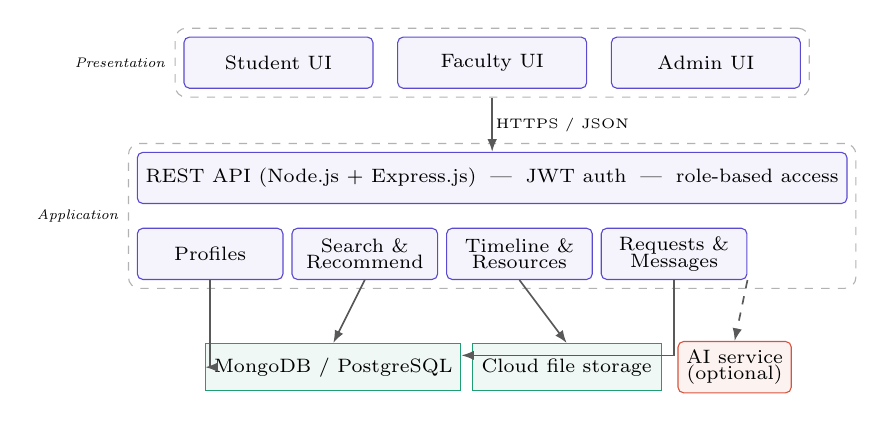
\begin{tikzpicture}[node distance=4mm and 3mm]
\node[box,minimum width=2.4cm] (s) {Student UI};
\node[box,right=of s,minimum width=2.4cm] (f) {Faculty UI};
\node[box,right=of f,minimum width=2.4cm] (a) {Admin UI};
\node[draw=black!30,dashed,rounded corners,fit=(s)(f)(a),inner sep=3pt,label={[font=\tiny\itshape]left:Presentation}] (pt) {};
\node[box,below=8mm of f,minimum width=7.9cm] (api) {REST API (Node.js + Express.js) \;|\; JWT auth \;|\; role-based access};
\node[box,below=3mm of api.south west,anchor=north west,minimum width=1.85cm] (m1) {Profiles};
\node[box,right=1mm of m1,minimum width=1.85cm] (m2) {Search \&\\[-2pt]Recommend};
\node[box,right=1mm of m2,minimum width=1.85cm] (m3) {Timeline \&\\[-2pt]Resources};
\node[box,right=1mm of m3,minimum width=1.85cm] (m4) {Requests \&\\[-2pt]Messages};
\node[draw=black!30,dashed,rounded corners,fit=(api)(m1)(m4),inner sep=3pt,label={[font=\tiny\itshape]left:Application}] (at) {};
\node[store,below=8mm of m2,minimum width=2.6cm,xshift=-4mm] (db) {MongoDB / PostgreSQL};
\node[store,below=8mm of m3,minimum width=2.4cm,xshift=6mm] (fs) {Cloud file storage};
\node[ext,right=2mm of fs,minimum width=1.4cm] (ai) {AI service\\[-2pt](optional)};
\draw[arr] (pt.south) -- node[lbl,right]{HTTPS / JSON} (api.north);
\draw[arr] (m2.south) -- (db.north); \draw[arr] (m1.south) |- (db.west);
\draw[arr] (m3.south) -- (fs.north); \draw[arr] (m4.south) |- ([yshift=1.5mm]db.east);
\draw[arr,dashed] (m4.south east) -- (ai.north);
\end{tikzpicture}}
\caption{Proposed three-tier production architecture.}
\label{fig:arch}
\end{figure}

\subsection{Prototype Architecture}
To validate the design quickly, the prototype is implemented as a client-side single-page application in one HTML file (HTML5, CSS3 and vanilla JavaScript) with no build step. A hash-based router maps addresses such as \texttt{\#/faculty/komal-bharti/work} to view renderers. Persistence and live features are provided through optional \emph{capabilities}: a shared document database with real-time snapshots, a presence channel, and an AI sampling interface. Each capability is requested inside a \texttt{try/catch}; when it is unavailable, as on plain static hosting, the application falls back to the browser's \texttt{localStorage} and rule-based logic (Fig.~\ref{fig:proto}). This mirrors the production separation of concerns while keeping hosting trivial.

\begin{figure}[t]
\centering
\resizebox{0.86\columnwidth}{!}{%
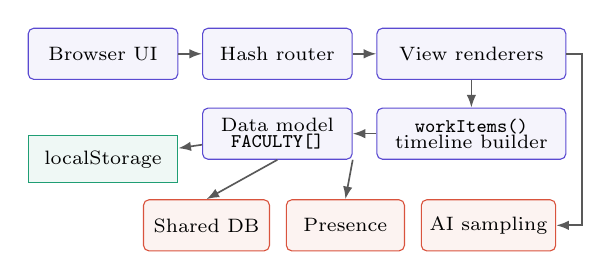
\begin{tikzpicture}[node distance=3.5mm and 3mm]
\node[box,minimum width=1.9cm] (ui) {Browser UI};
\node[box,right=of ui,minimum width=1.9cm] (rt) {Hash router};
\node[box,right=of rt,minimum width=2.4cm] (vw) {View renderers};
\node[box,below=of rt,minimum width=1.9cm] (dm) {Data model\\[-2pt]\texttt{FACULTY[]}};
\node[box,below=of vw,minimum width=2.4cm] (tl) {\texttt{workItems()}\\[-2pt]timeline builder};
\node[store,below=7mm of ui,minimum width=1.9cm] (ls) {localStorage};
\node[ext,below=5mm of dm,minimum width=1.6cm,xshift=-9mm] (db) {Shared DB};
\node[ext,right=2mm of db,minimum width=1.5cm] (pr) {Presence};
\node[ext,right=2mm of pr,minimum width=1.6cm] (ai) {AI sampling};
\draw[arr] (ui)--(rt); \draw[arr] (rt)--(vw); \draw[arr] (vw)--(tl); \draw[arr] (tl)--(dm);
\draw[arr] (dm)--(ls); \draw[arr] (dm.south)--(db.north); \draw[arr] (dm.south east)--(pr.north);
\draw[arr] (vw.east) -- ++(2mm,0) |- (ai.east);
\end{tikzpicture}}
\caption{Prototype runtime architecture; red components are optional and fall back gracefully.}
\label{fig:proto}
\end{figure}

\subsection{Use-Case Model}
Fig.~\ref{fig:usecase} shows the principal use cases for the three actors.

\begin{figure}[t]
\centering
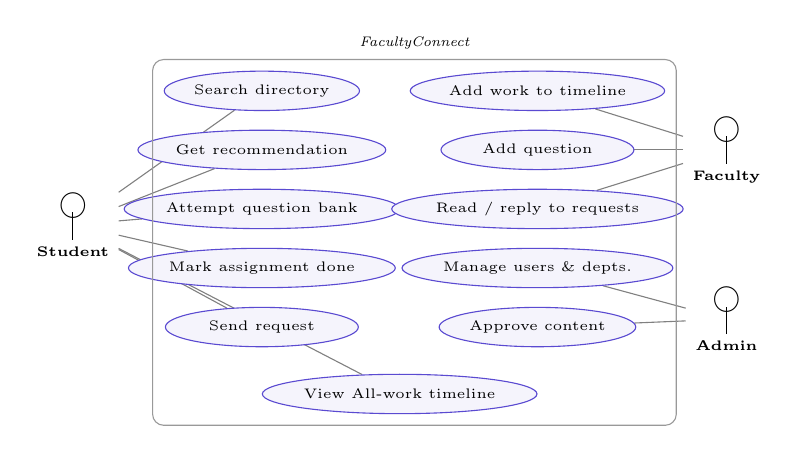
\begin{tikzpicture}[font=\scriptsize,
  uc/.style={ellipse,draw=brand,fill=brand!6,minimum width=2.45cm,minimum height=5mm,inner sep=0.5pt,font=\tiny},
  actor/.style={align=center,font=\tiny\bfseries}]
\node[actor] (stu) at (0,0.3) {\normalsize$\bigcirc$\\[-3pt]\rule{0.4pt}{3.5mm}\\Student};
\node[actor] (fac) at (8.3,1.25) {\normalsize$\bigcirc$\\[-3pt]\rule{0.4pt}{3.5mm}\\Faculty};
\node[actor] (adm) at (8.3,-0.9) {\normalsize$\bigcirc$\\[-3pt]\rule{0.4pt}{3.5mm}\\Admin};
\node[uc] (u1) at (2.4,2.0) {Search directory};
\node[uc] (u2) at (2.4,1.25) {Get recommendation};
\node[uc] (u3) at (2.4,0.5) {Attempt question bank};
\node[uc] (u4) at (2.4,-0.25) {Mark assignment done};
\node[uc] (u5) at (2.4,-1.0) {Send request};
\node[uc] (u0) at (4.15,-1.85) {View All-work timeline};
\node[uc] (u6) at (5.9,2.0) {Add work to timeline};
\node[uc] (u7) at (5.9,1.25) {Add question};
\node[uc] (u8) at (5.9,0.5) {Read / reply to requests};
\node[uc] (u9) at (5.9,-0.25) {Manage users \& depts.};
\node[uc] (u10) at (5.9,-1.0) {Approve content};
\node[draw=black!40,rounded corners,fit=(u1)(u0)(u6)(u10),inner sep=4pt,label={[font=\tiny\itshape]above:FacultyConnect}] {};
\begin{scope}[on background layer]
\foreach \u in {u1,u2,u3,u4,u5,u0} \draw[black!50] (stu)--(\u);
\foreach \u in {u6,u7,u8} \draw[black!50] (fac)--(\u);
\foreach \u in {u9,u10} \draw[black!50] (adm)--(\u);
\end{scope}
\end{tikzpicture}
\caption{Use-case diagram.}
\label{fig:usecase}
\end{figure}

\subsection{Data-Flow Model}
The level-0 data-flow diagram (Fig.~\ref{fig:dfd}) shows the system as a single process exchanging data with the three external entities. At level~1 the process decomposes into: P1 Authentication, P2 Search and Recommendation, P3 Profile and Timeline Management, P4 Assessment (assignments and question bank) and P5 Messaging, with data stores D1 Users, D2 Faculty Profiles, D3 Work Items, D4 Questions and D5 Messages.

\begin{figure}[t]
\centering
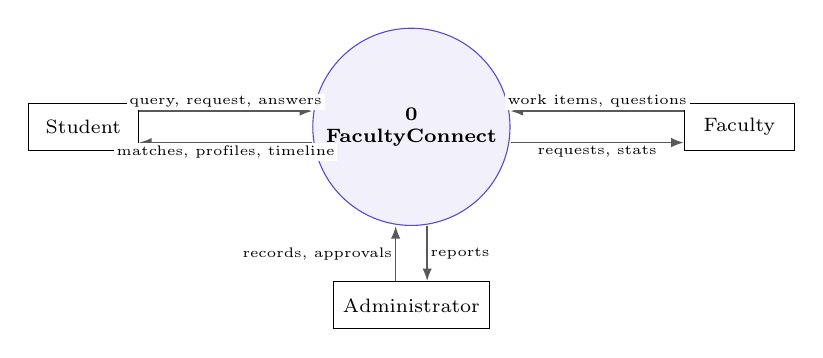
\begin{tikzpicture}[node distance=5mm]
\node[circle,draw=brand,fill=brand!8,minimum size=15mm,align=center,font=\scriptsize\bfseries] (p) {0\\FacultyConnect};
\node[draw,minimum width=1.4cm,minimum height=6mm,font=\scriptsize,left=2.2cm of p] (s) {Student};
\node[draw,minimum width=1.4cm,minimum height=6mm,font=\scriptsize,right=2.2cm of p] (f) {Faculty};
\node[draw,minimum width=1.4cm,minimum height=6mm,font=\scriptsize,below=7mm of p] (a) {Administrator};
\draw[arr] ([yshift=2mm]s.east) -- node[lbl,above]{query, request, answers} ([yshift=2mm]p.west);
\draw[arr] ([yshift=-2mm]p.west) -- node[lbl,below]{matches, profiles, timeline} ([yshift=-2mm]s.east);
\draw[arr] ([yshift=2mm]f.west) -- node[lbl,above]{work items, questions} ([yshift=2mm]p.east);
\draw[arr] ([yshift=-2mm]p.east) -- node[lbl,below]{requests, stats} ([yshift=-2mm]f.west);
\draw[arr] ([xshift=-2mm]a.north) -- node[lbl,left]{records, approvals} ([xshift=-2mm]p.south);
\draw[arr] ([xshift=2mm]p.south) -- node[lbl,right]{reports} ([xshift=2mm]a.north);
\end{tikzpicture}
\caption{Level-0 data-flow (context) diagram.}
\label{fig:dfd}
\end{figure}

\subsection{Entity--Relationship Model}
Fig.~\ref{fig:er} shows the main entities. A \textsc{Department} has many \textsc{Faculty}; a \textsc{Faculty} teaches many \textsc{Course}s and owns many \textsc{WorkItem}s, \textsc{Question}s and incoming \textsc{Request}s; a \textsc{Student} sends many \textsc{Request}s and records many \textsc{Progress} entries. \textsc{WorkItem} is a generalization whose \emph{type} attribute takes the values lecture, video, solutions, paper, project or assignment; the \emph{date} attribute orders the timeline.

\begin{figure}[t]
\centering
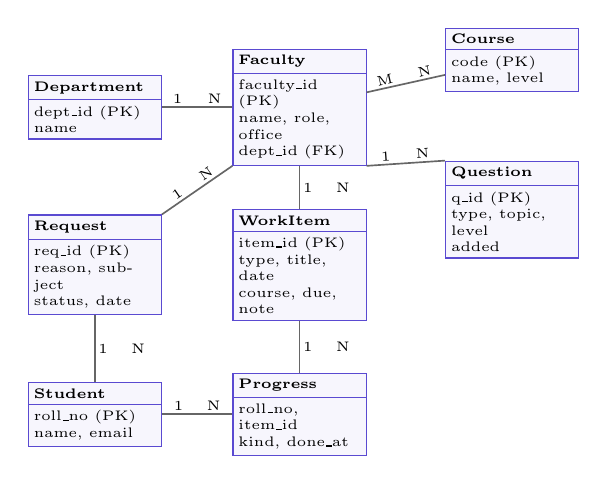
\begin{tikzpicture}[font=\tiny,
  ent/.style={rectangle split,rectangle split parts=2,draw=brand,fill=brand!5,font=\tiny,align=left,inner sep=2pt,text width=1.55cm},
  rel/.style={-,semithick,draw=black!60},
  card/.style={font=\tiny,inner sep=1pt}]
\node[ent] (dep) at (0,0) {\textbf{Department}\nodepart{second}dept\_id (PK)\\name};
\node[ent] (fac) at (2.6,0) {\textbf{Faculty}\nodepart{second}faculty\_id (PK)\\name, role, office\\dept\_id (FK)};
\node[ent] (crs) at (5.3,0.6) {\textbf{Course}\nodepart{second}code (PK)\\name, level};
\node[ent] (wi)  at (2.6,-2.0) {\textbf{WorkItem}\nodepart{second}item\_id (PK)\\type, title, date\\course, due, note};
\node[ent] (q)   at (5.3,-1.3) {\textbf{Question}\nodepart{second}q\_id (PK)\\type, topic, level\\added};
\node[ent] (req) at (0,-2.0) {\textbf{Request}\nodepart{second}req\_id (PK)\\reason, subject\\status, date};
\node[ent] (stu) at (0,-3.9) {\textbf{Student}\nodepart{second}roll\_no (PK)\\name, email};
\node[ent] (pg)  at (2.6,-3.9) {\textbf{Progress}\nodepart{second}roll\_no, item\_id\\kind, done\_at};
\draw[rel] (dep) -- node[card,above]{1 \quad N} (fac);
\draw[rel] (fac) -- node[card,above,sloped]{M \quad N} (crs);
\draw[rel] (fac) -- node[card,right]{1 \;\; N} (wi);
\draw[rel] (fac.south east) -- node[card,above,sloped]{1 \quad N} (q.north west);
\draw[rel] (fac.south west) -- node[card,above,sloped]{1 \;\; N} (req.north east);
\draw[rel] (stu) -- node[card,right]{1 \;\; N} (req);
\draw[rel] (stu) -- node[card,above]{1 \;\; N} (pg);
\draw[rel] (wi) -- node[card,right]{1 \;\; N} (pg);
\end{tikzpicture}
\caption{Entity--relationship model (simplified).}
\label{fig:er}
\end{figure}

\subsection{Sequence of Adding Work}
Fig.~\ref{fig:seq} shows the interaction when a faculty member adds an item. The form handler builds the item, the model appends it, the persistence layer writes it locally and to the shared database, and every subscribed client re-renders the timeline from its snapshot listener.

\begin{figure}[t]
\centering
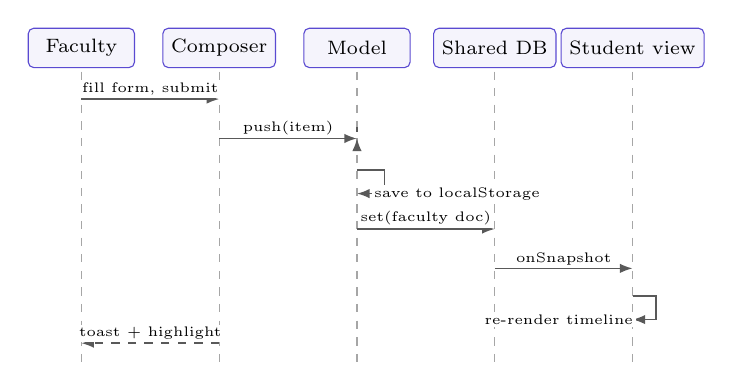
\begin{tikzpicture}[font=\tiny]
\foreach \x/\n/\t in {0/f/Faculty,1.75/ui/Composer,3.5/m/Model,5.25/db/Shared DB,7.0/v/Student view}{
  \node[box,minimum width=1.35cm,minimum height=5mm] (\n) at (\x,0) {\t};
  \draw[black!35,dashed] (\x,-0.3) -- (\x,-4.0);}
\def\msg#1#2#3#4{\draw[arr] (#1,#3) -- node[lbl,above]{#4} (#2,#3);}
\msg{0}{1.75}{-0.65}{fill form, submit}
\msg{1.75}{3.5}{-1.15}{push(item)}
\msg{3.5}{3.5}{-1.15}{}
\draw[arr] (3.5,-1.55) -- ++(0.35,0) -- ++(0,-0.3) -- node[lbl,right]{save to localStorage} (3.5,-1.85);
\msg{3.5}{5.25}{-2.3}{set(faculty doc)}
\msg{5.25}{7.0}{-2.8}{onSnapshot}
\draw[arr] (7.0,-3.15) -- ++(0.3,0) -- ++(0,-0.3) -- node[lbl,left,xshift=-1mm]{re-render timeline} (7.0,-3.45);
\draw[arr,dashed] (1.75,-3.75) -- node[lbl,above]{toast + highlight} (0,-3.75);
\end{tikzpicture}
\caption{Sequence diagram: adding an item to the All work timeline.}
\label{fig:seq}
\end{figure}

% =====================================================================
\section{Implementation}

\subsection{Technology Stack}
Table~\ref{tab:stack} contrasts the proposed production stack with the stack used for the deployed prototype.

\begin{table}[t]
\caption{Technology Stack}
\label{tab:stack}
\centering\scriptsize
\begin{tabularx}{\columnwidth}{@{}l Y Y@{}}
\toprule
\textbf{Component} & \textbf{Proposed (production)} & \textbf{Prototype (deployed)}\\
\midrule
Frontend & React.js, Tailwind CSS & HTML5, CSS3, vanilla JavaScript (ES2020)\\
Backend & Node.js, Express.js REST API & Client-side logic; no server code\\
Database & MongoDB / PostgreSQL & Shared document DB (optional) + localStorage\\
Authentication & JWT, role-based access & Simulated role picker\\
Search & Keyword / skill-overlap scoring & Same, plus optional LLM ranking\\
Storage & Cloud object storage & Data URL on device ($\le$1.5\,MB)\\
Real-time & WebSockets & Snapshot listeners, presence channel\\
Hosting & Cloud VM / PaaS & Vercel static hosting\\
Testing & Jest, Playwright & Playwright (headless Chromium)\\
\bottomrule
\end{tabularx}
\end{table}

\subsection{Module Overview}
\begin{itemize}
  \item \textbf{Router:} \texttt{navigate()} and \texttt{doRenderRoute()} select the view, apply animated view transitions, and ensure only one upload form exists in the page at a time.
  \item \textbf{Directory:} full-text match across name, department, role, research areas and publication titles, plus department filter chips.
  \item \textbf{Profile:} \texttt{profileTabHTML()} renders nine tabs; old links to the former \emph{Lectures} tab redirect to \emph{All work}.
  \item \textbf{Timeline:} \texttt{workItems()}, \texttt{workTimelineHTML()}, \texttt{wireWorkForm()} and \texttt{openWorkItem()}.
  \item \textbf{Assessment:} assignment status and completion, MCQ checking, answer reveal, faculty authoring and AI question generation.
  \item \textbf{Messaging:} contact form, faculty inbox, toast and bell badge driven by snapshot changes.
  \item \textbf{Recommendation and helpdesk:} language-model prompts returning structured JSON, with keyword-scoring and pattern-matched fallbacks.
\end{itemize}

\subsection{Unified All Work Timeline}
In the first prototype, files a faculty member uploaded appeared in a separate ``Your uploads'' box on the dashboard and again as an ``Uploaded resources'' list beneath lecture units, while assignments and questions lived in other tabs and no item showed when it had been shared. Following review feedback, these were merged into a single derived timeline. The timeline is not stored; it is computed from the existing collections each time it is rendered, which keeps a single source of truth (Algorithm~\ref{alg:timeline}).

\begin{algorithm}[t]
\caption{Building the All Work timeline}
\label{alg:timeline}
\small
\begin{algorithmic}[1]
\Require faculty record $f$, type filter $t$
\State $I \gets \emptyset$
\ForAll{$u \in f.\mathit{uploads}$} \State $I \gets I \cup \{(u.\mathit{type}, u.\mathit{title}, \textsc{ToDate}(u.\mathit{date}))\}$ \EndFor
\ForAll{$a \in f.\mathit{assignments}$} \State $I \gets I \cup \{(\text{assignment}, a.\mathit{title}, \textsc{ToDate}(a.\mathit{posted}))\}$ \EndFor
\ForAll{$l \in f.\mathit{lectures}$} \State $I \gets I \cup \{(\text{lecture}, l.\mathit{title}, \textsc{ToDate}(l.\mathit{posted}))\}$ \EndFor
\ForAll{$q \in f.\mathit{questions}$} \State $I \gets I \cup \{(\text{question}, q.\mathit{text}, \textsc{ToDate}(q.\mathit{added}))\}$ \EndFor
\State sort $I$ by date, descending
\If{$t \neq$ all} \State $I \gets \{i \in I : i.\mathit{type} = t\}$ \EndIf
\State partition $I$ into consecutive groups of equal (year, month)
\State \Return groups for rendering
\end{algorithmic}
\end{algorithm}

Each row shows a day/month date tile, a coloured type badge, course code, relative date (``Today'', ``Yesterday'' or a full date), due date and open/closed status for assignments, live view count, and attached file name. Filter chips show the count per type. The composer, available both on the faculty dashboard and inside the faculty member's own \emph{All work} tab, writes to the same list; the new row is highlighted as ``just added''. A \emph{Date shared} field lets faculty add older material, which is placed in the correct month instead of at the top. \textsc{ToDate} accepts ISO dates, month--year strings (``Jul 2026''), day--month--year strings (``20 Sep 2026'') and legacy ``just now'' values, so data saved by earlier versions still sorts correctly. Sorting dominates the cost, giving $O(n\log n)$ time for $n$ items, which is negligible for the few hundred items a faculty member shares in a year.

\subsection{Faculty Recommendation}
Let $W(q)$ be the set of words longer than three characters in the student's query $q$, and let $R_f$ be the research areas of faculty member $f$, each with a name and description $\mathrm{text}(r)$. The baseline score is
\begin{equation}
s(f,q) \;=\; \max_{r\in R_f} \sum_{w\in W(q)} \mathbb{1}\big[\,w \sqsubseteq \mathrm{text}(r)\,\big],
\end{equation}
where $w \sqsubseteq \mathrm{text}(r)$ denotes that $w$ occurs in the lower-cased text. Faculty with $s>0$ are ranked by score and the top three are returned; the best-matching area $r^{*}$ provides the explanation shown to the student (``Works on \emph{devops-ci} --- build failure prediction and pipeline optimization''). When the AI capability is present, the faculty list and query are sent to a language model that returns a JSON array of identifiers and reasons; identifiers are validated against the faculty list before display, so the model cannot introduce non-existent faculty. If neither path yields a match, a well-rounded default profile is suggested.

\subsection{Data Persistence and Synchronization}
Every write calls \texttt{dbSyncFaculty()}, which first saves all faculty data to \texttt{localStorage} and then, if the shared database is available, writes the faculty document. Each client subscribes to every faculty document; on a snapshot it replaces the in-memory collections and re-renders only the affected view. If the browser storage quota is exceeded, embedded file contents are dropped and metadata retained. File contents are never sent to the shared database, keeping documents small.

\subsection{Security Considerations}
All user-entered text shown in the timeline and assignments is passed through an escaping function that replaces \verb|& < > " '| with HTML entities, preventing stored cross-site scripting. Faculty-only actions are shown only when the signed-in faculty member manages the profile being viewed. In production these checks move to the API layer, where JWTs carry the role and profile identifier.

% =====================================================================
\section{Prototype Interface}

The interface uses a dark theme with a per-department accent colour, large tap targets, animated counters and page transitions, and a command palette (Ctrl+K) for quick navigation. Fig.~\ref{fig:mock} shows the initial interface concept and Fig.~\ref{fig:screens} the implemented screens.

\begin{figure}[t]
\centering
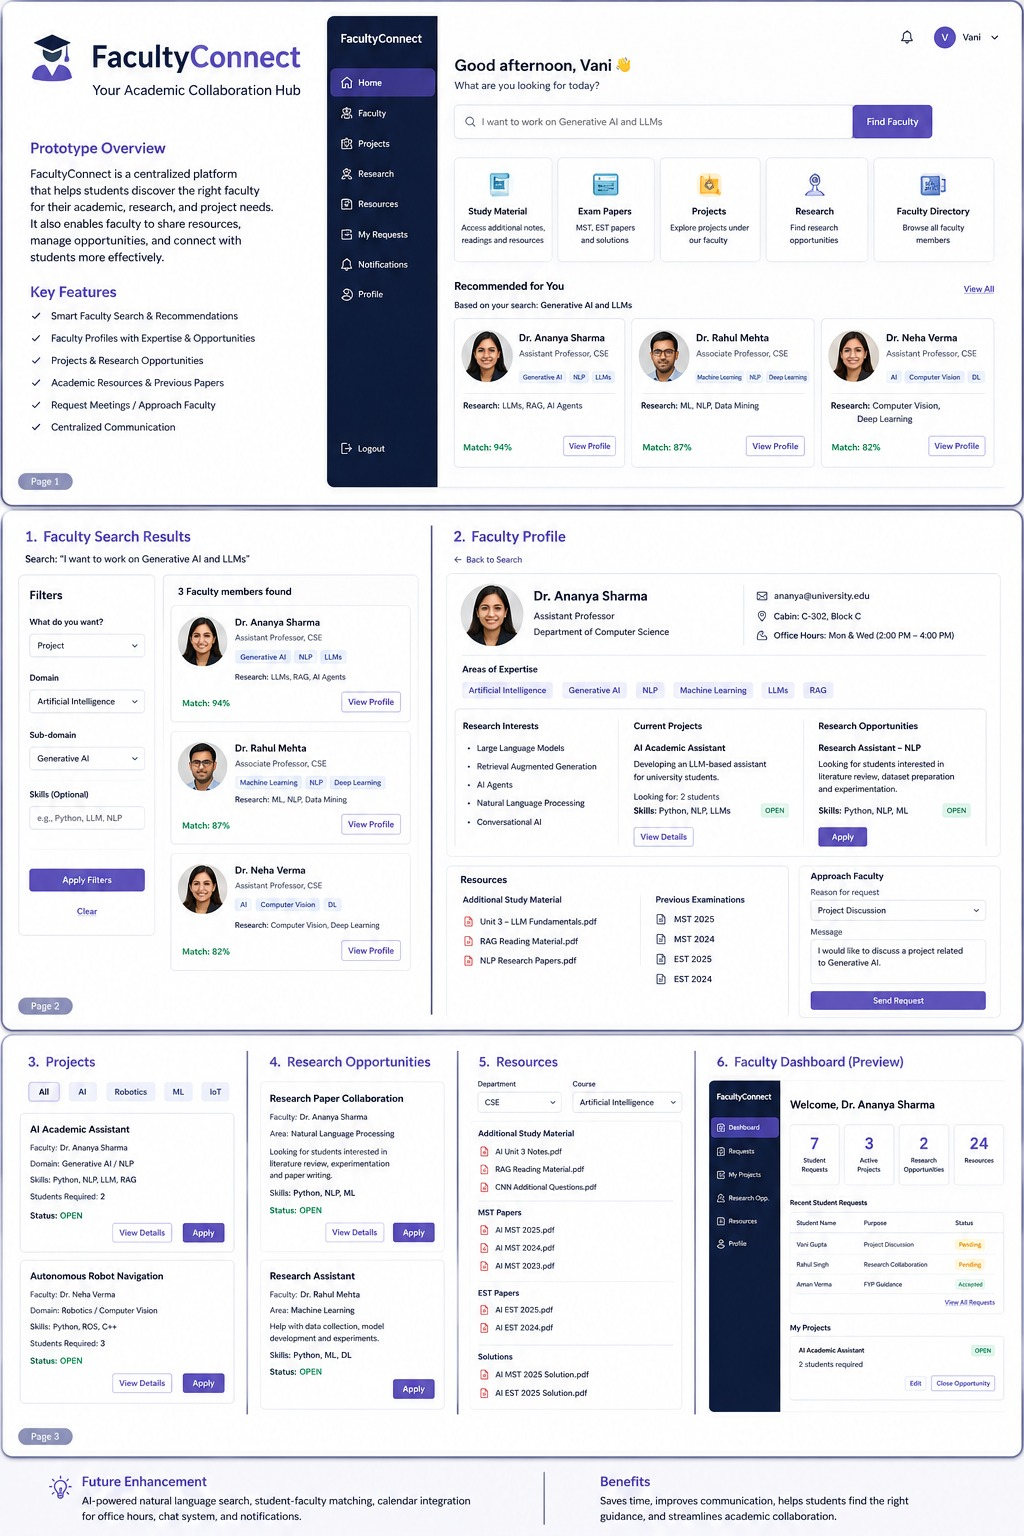
\includegraphics[width=0.78\columnwidth]{figures/prototype_mockup.jpg}
\caption{Initial interface concept prepared during requirement analysis.}
\label{fig:mock}
\end{figure}

\begin{figure*}[t]
\centering
\begin{minipage}{0.325\textwidth}\centering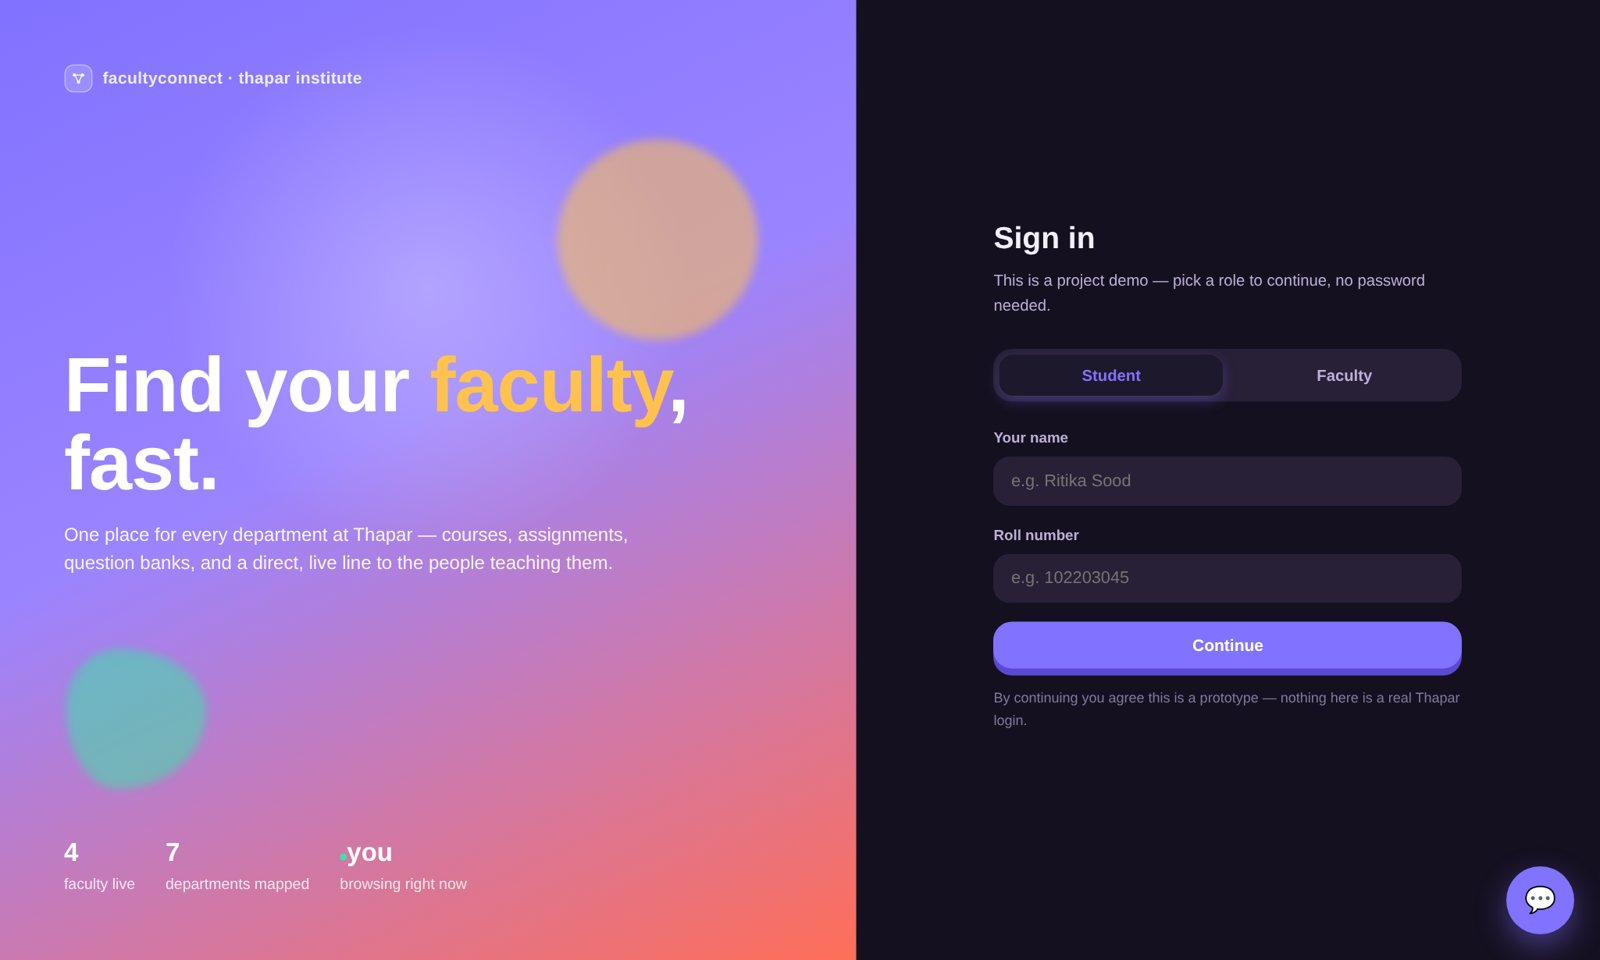
\includegraphics[width=\linewidth]{figures/login.jpg}\\[-1pt]{\scriptsize (a) Role-based sign-in}\end{minipage}\hfill
\begin{minipage}{0.325\textwidth}\centering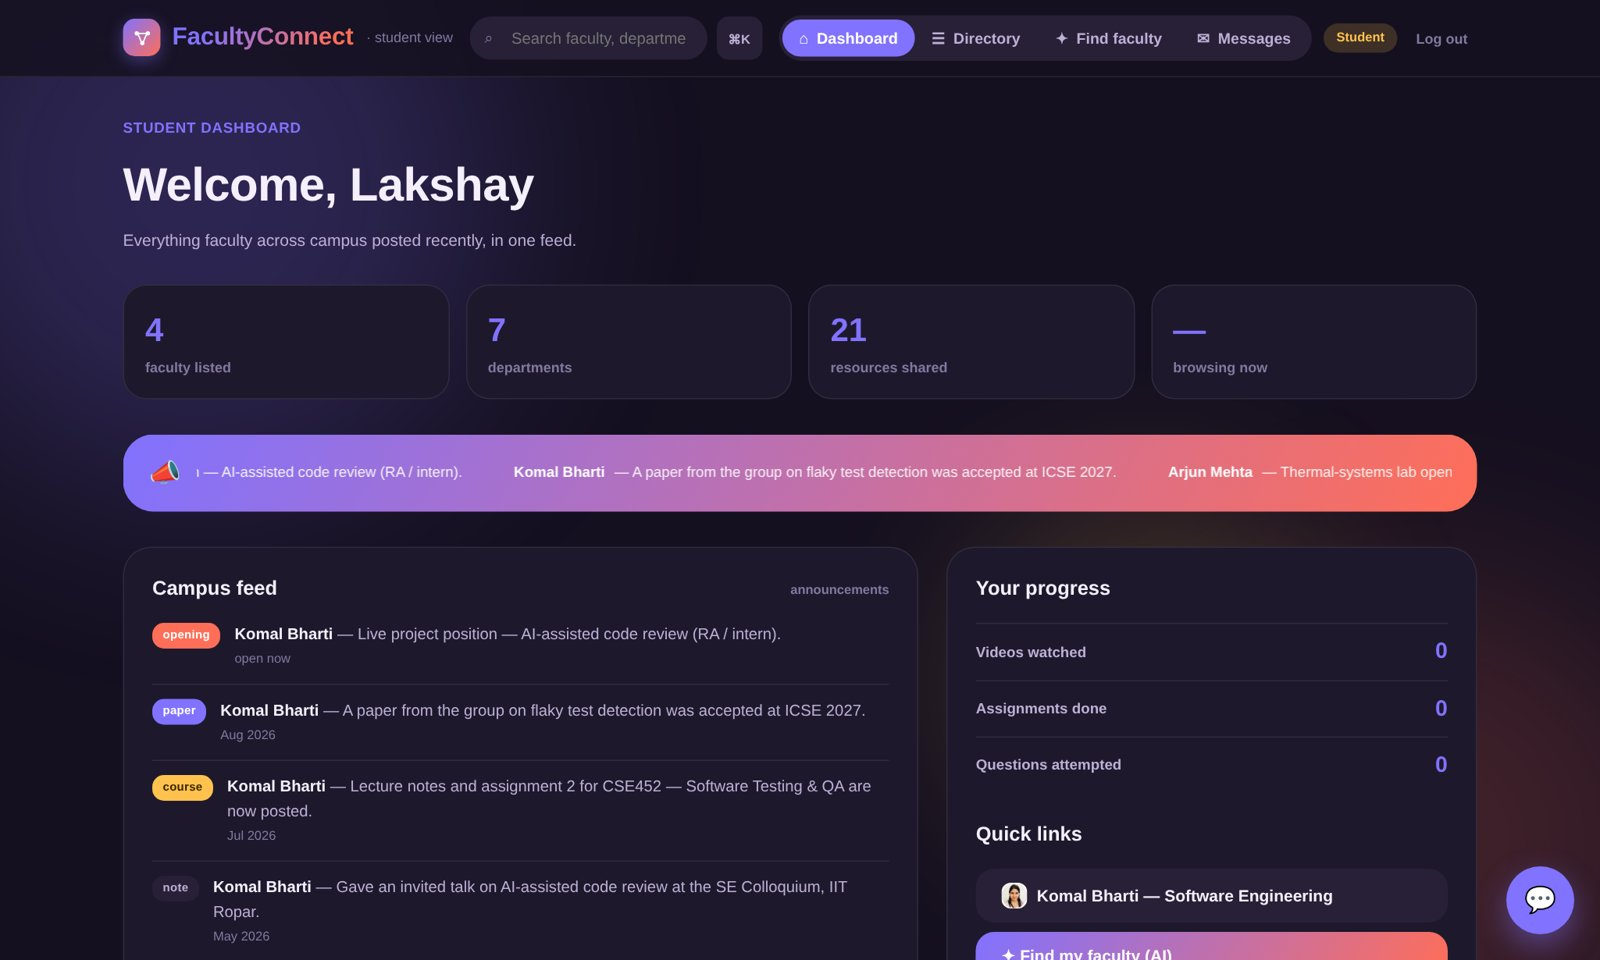
\includegraphics[width=\linewidth]{figures/dashboard-student.jpg}\\[-1pt]{\scriptsize (b) Student dashboard}\end{minipage}\hfill
\begin{minipage}{0.325\textwidth}\centering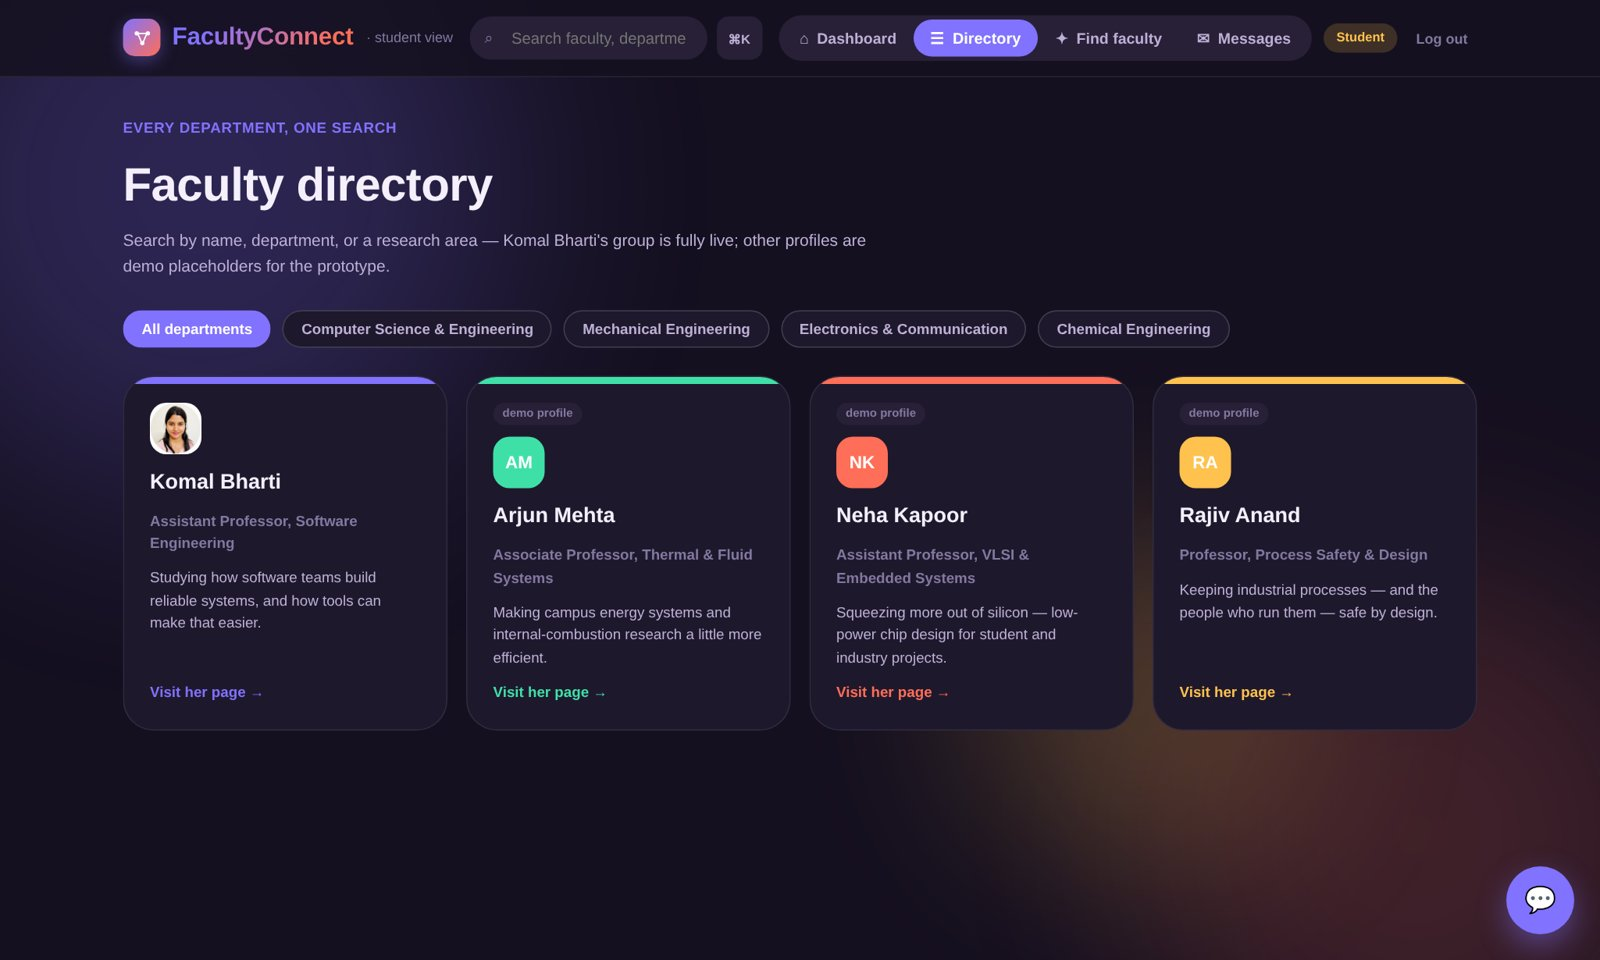
\includegraphics[width=\linewidth]{figures/directory.jpg}\\[-1pt]{\scriptsize (c) Faculty directory}\end{minipage}\\[5pt]
\begin{minipage}{0.325\textwidth}\centering
\includegraphics[width=\linewidth]{figures/profile.jpg}\\[-1pt]{\scriptsize (d) Faculty profile}\end{minipage}\hfill
\begin{minipage}{0.325\textwidth}\centering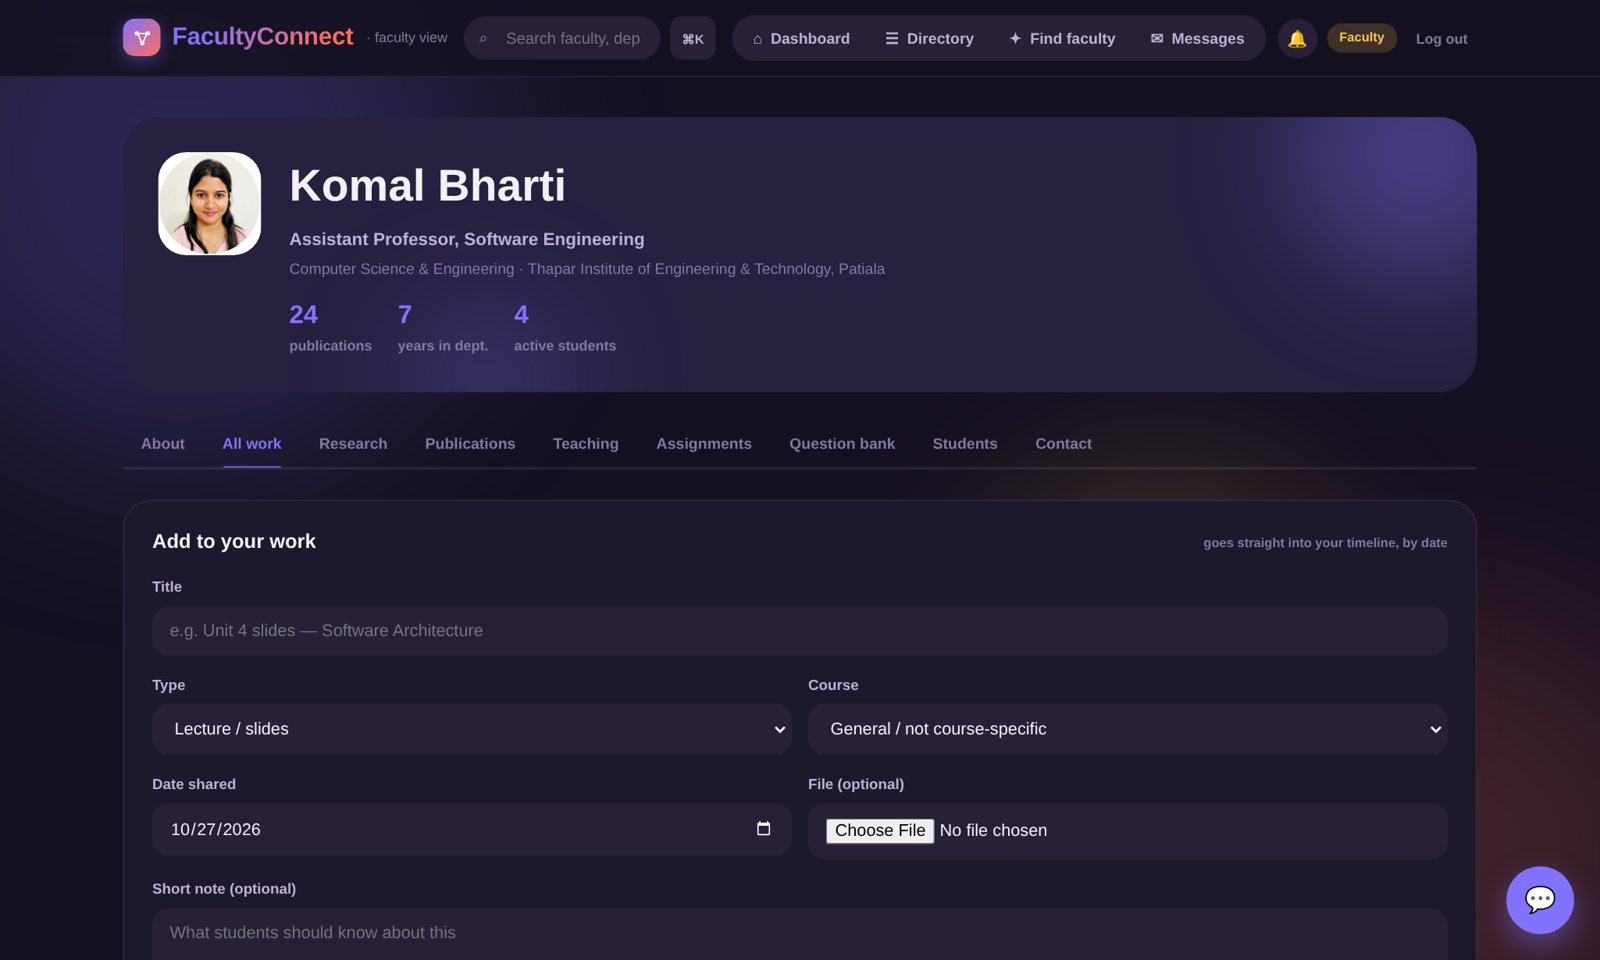
\includegraphics[width=\linewidth]{figures/composer.jpg}\\[-1pt]{\scriptsize (e) Adding work to the timeline}\end{minipage}\hfill
\begin{minipage}{0.325\textwidth}\centering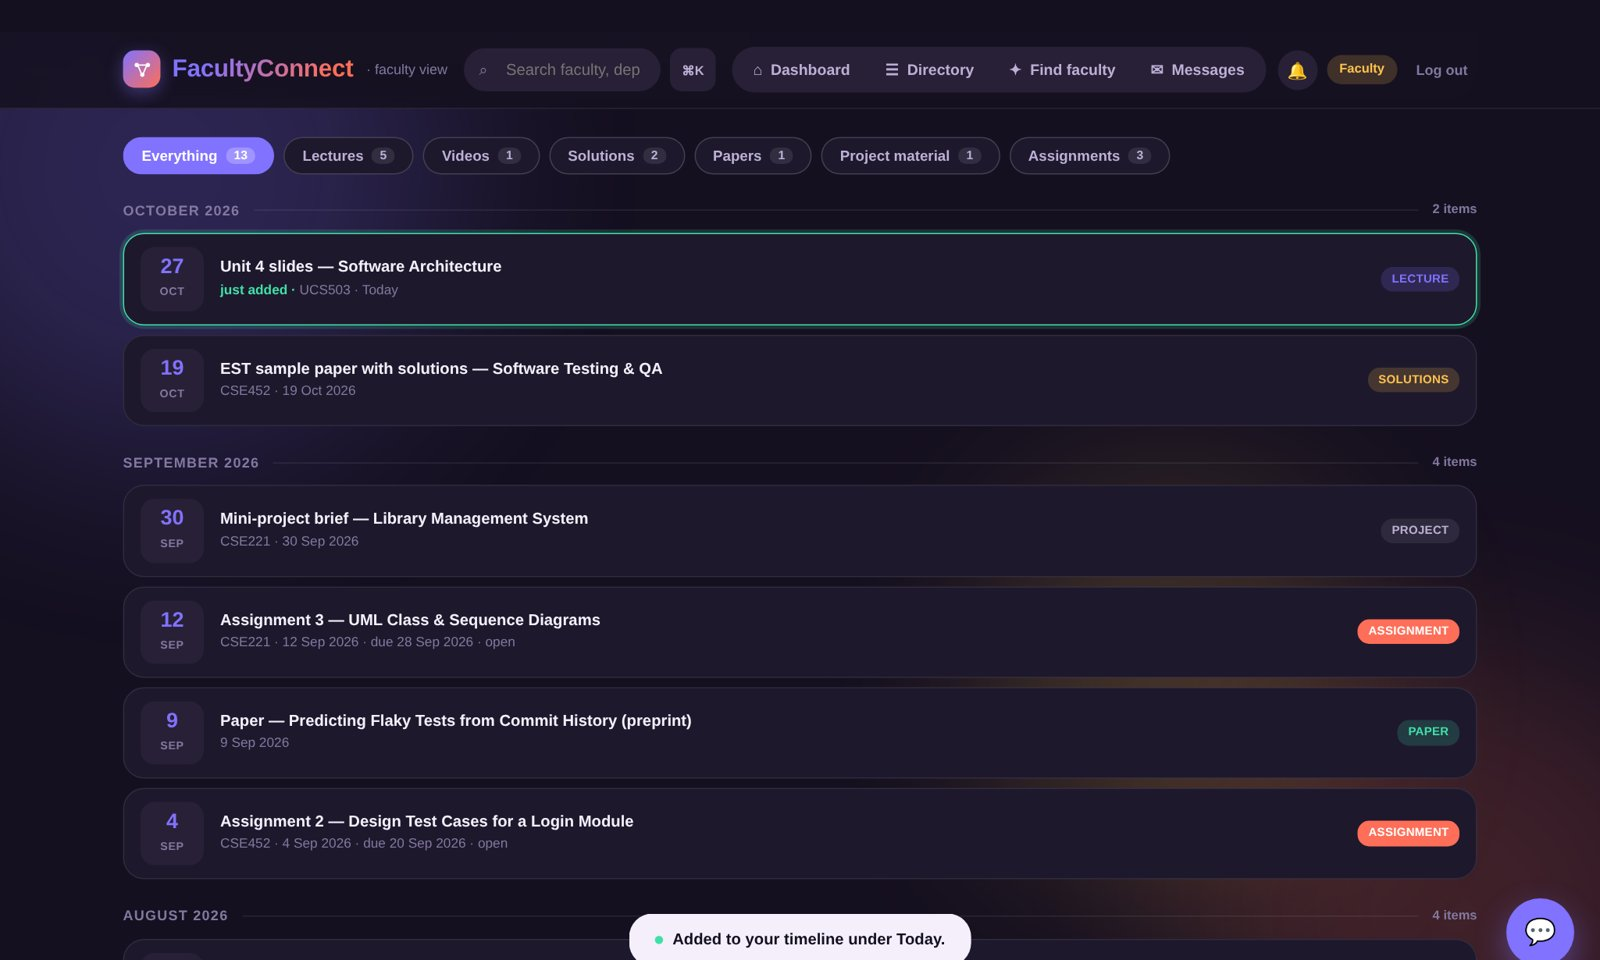
\includegraphics[width=\linewidth]{figures/timeline.jpg}\\[-1pt]{\scriptsize (f) All work timeline, grouped by month}\end{minipage}\\[5pt]
\begin{minipage}{0.325\textwidth}\centering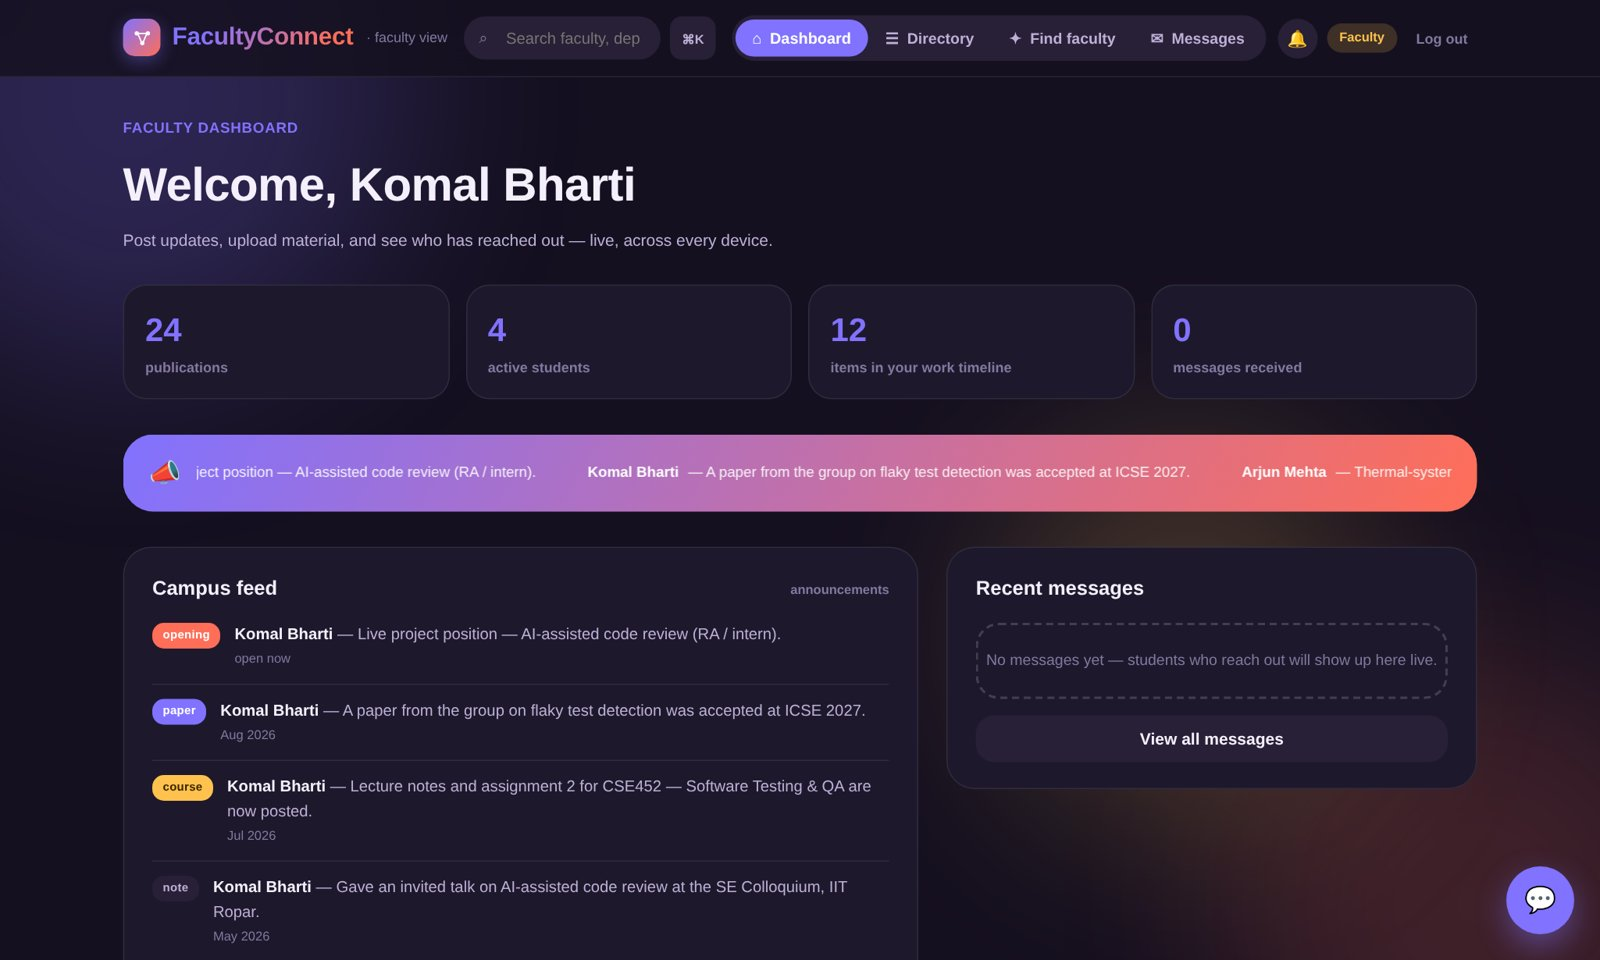
\includegraphics[width=\linewidth]{figures/dashboard-faculty.jpg}\\[-1pt]{\scriptsize (g) Faculty dashboard}\end{minipage}\hfill
\begin{minipage}{0.325\textwidth}\centering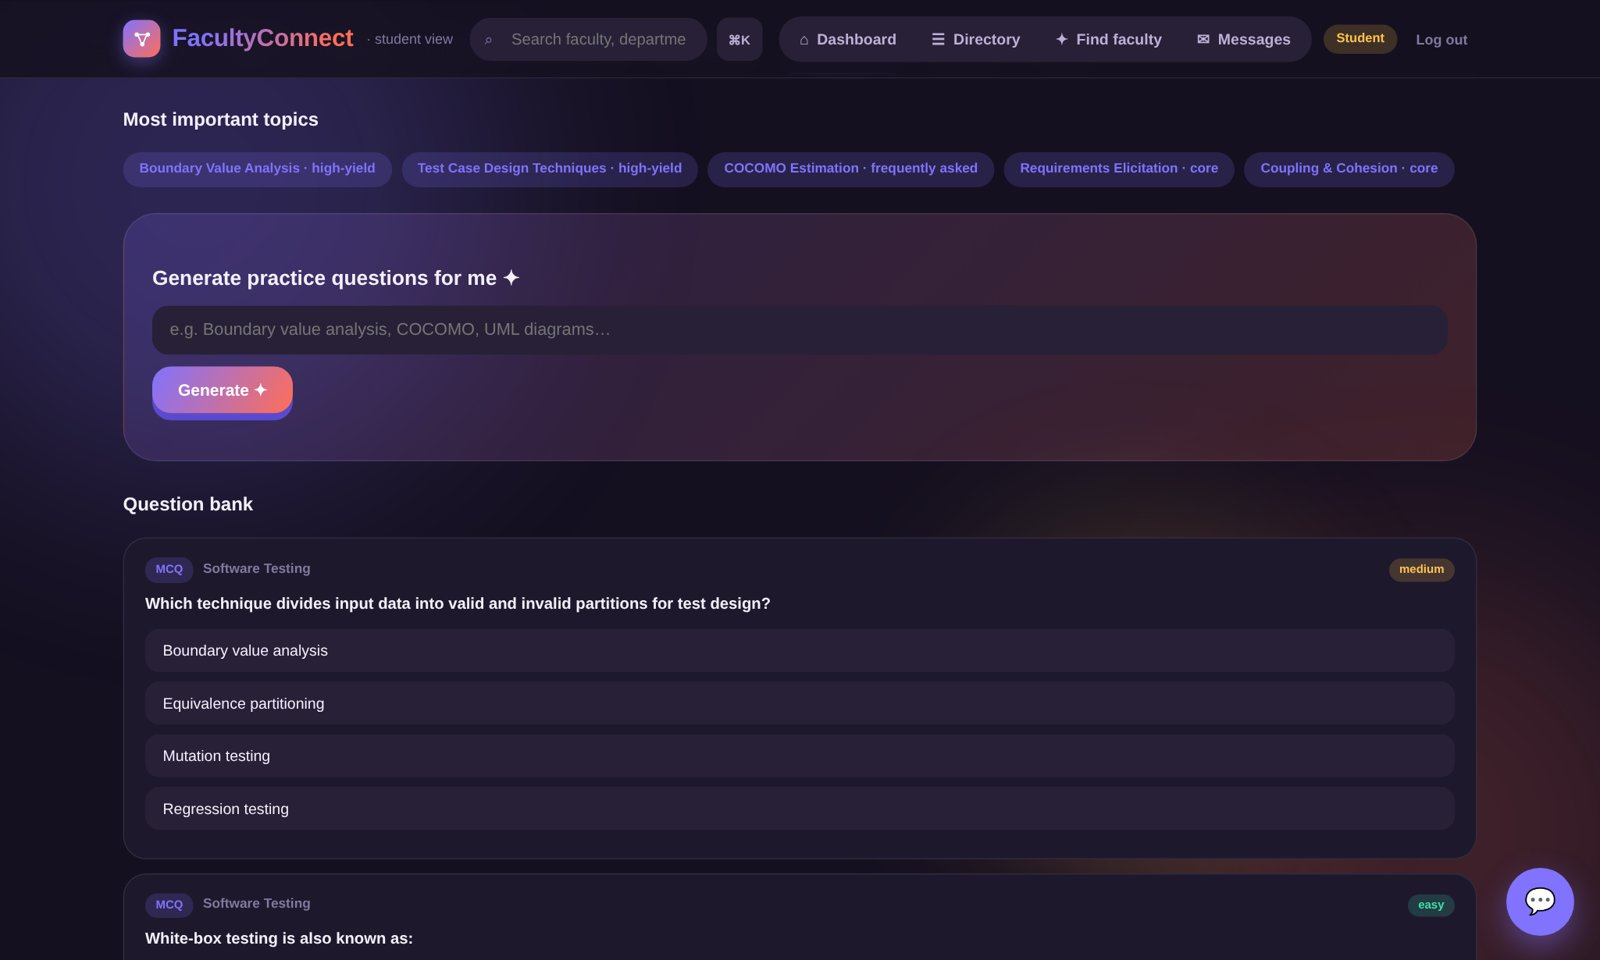
\includegraphics[width=\linewidth]{figures/questionbank.jpg}\\[-1pt]{\scriptsize (h) Interactive question bank}\end{minipage}\hfill
\begin{minipage}{0.325\textwidth}\centering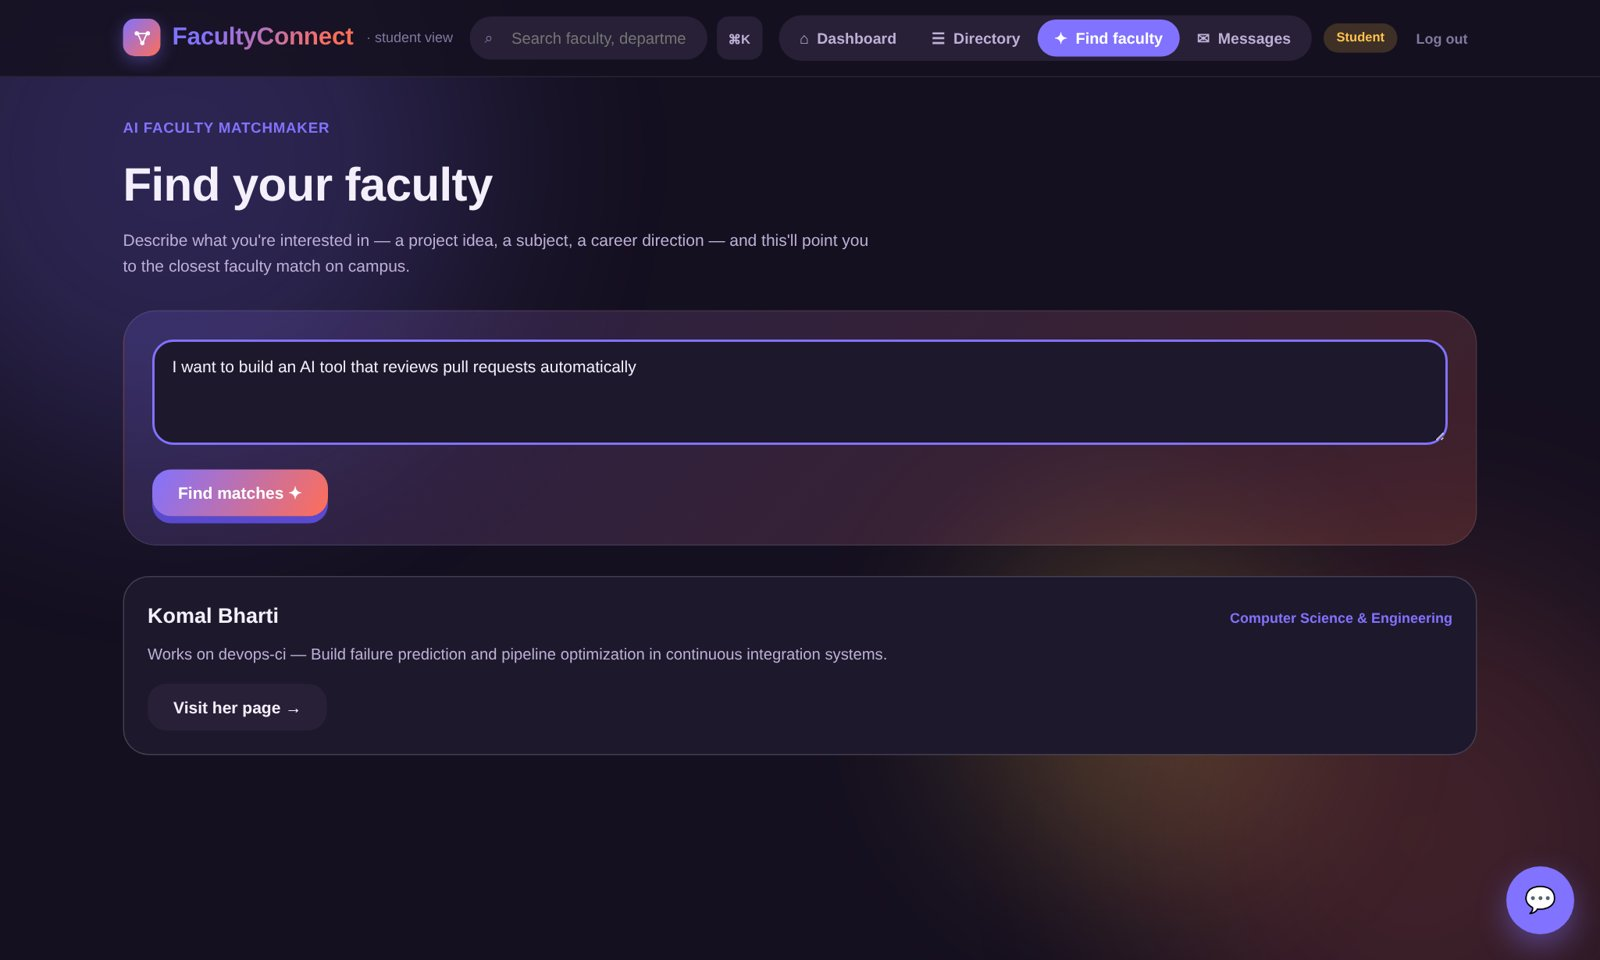
\includegraphics[width=\linewidth]{figures/match.jpg}\\[-1pt]{\scriptsize (i) Faculty recommendation}\end{minipage}
\caption{Implemented FacultyConnect prototype screens.}
\label{fig:screens}
\end{figure*}

\subsection{Student Journey}
After signing in (Fig.~\ref{fig:screens}a), the student dashboard (b) shows statistics, a scrolling announcement ticker, a campus feed and a personal progress panel. The directory (c) lists faculty cards coloured by department. A profile (d) opens on the About tab; the \emph{All work} tab (f) lists everything that faculty member has shared, which the student can filter, for example to \emph{Solutions} before an examination. The question bank (h) gives instant feedback, and the recommendation page (i) suggests faculty for a free-text interest.

\subsection{Faculty Journey}
The faculty dashboard (g) shows publications, students, timeline items and messages received, followed by the composer (e) and the five most recent timeline items. Adding an item takes one form submission, after which a confirmation states the date under which it was filed.

% =====================================================================
\section{Testing}

\subsection{Test Strategy}
Testing combined (i) unit-level checks of pure functions such as \textsc{ToDate} and \texttt{workItems()}; (ii) black-box test cases designed with equivalence partitioning and boundary value analysis \cite{pressman}; (iii) automated end-to-end scenarios in headless Chromium using Playwright \cite{playwright}, which signed in as each role, submitted forms, applied filters and inspected the resulting page; and (iv) responsive checks at 360, 390 and 1366\,px widths.

\subsection{Test Cases}
Table~\ref{tab:tests} lists the executed test cases. All twelve passed after the fixes described below.

\begin{table*}[t]
\caption{Executed Test Cases}
\label{tab:tests}
\centering\footnotesize
\begin{tabularx}{\textwidth}{@{}l l Y Y l@{}}
\toprule
\textbf{ID} & \textbf{Technique} & \textbf{Input / action} & \textbf{Expected result} & \textbf{Result}\\
\midrule
T1 & Functional & Faculty adds item dated today & Appears first under current month, marked ``just added'' & Pass\\
T2 & Functional & Item back-dated to 10 Aug 2026 & Placed between the 18 Aug and 4 Aug entries & Pass\\
T3 & EP (invalid) & Submit with empty title & Submission blocked; no item created & Pass\\
T4 & EP (valid) & Assignment with due date 1 Dec 2026 & Status \emph{open} in timeline and Assignments tab & Pass\\
T5 & EP (valid) & Assignment with due date 1 Oct 2026 & Status \emph{closed} & Pass\\
T6 & Functional & Select \emph{Lectures} filter chip & Only lecture items shown; counts unchanged & Pass\\
T7 & Security & Title containing \verb|<script>| and \verb|<img onerror>| & Rendered as plain text; script not executed & Pass\\
T8 & Regression & Legacy saved data with dates ``just now'' and ``Jul 2026'' & Migrated and sorted correctly & Pass\\
T9 & Regression & Open old address \texttt{\#/faculty/id/lectures} & Redirects to \emph{All work} tab & Pass\\
T10 & BVA & Files of 1.5\,MB and 1.6\,MB (limit 1.5\,MB) & First stored for download; second keeps name only & Pass\\
T11 & Robustness & Run on static hosting with no database or AI & No errors; local storage and fallbacks used & Pass\\
T12 & Usability & Viewport 360\,px & No horizontal page scroll & Pass (after fix)\\
\bottomrule
\end{tabularx}
\end{table*}

\subsection{Defects Found and Fixed}
\begin{enumerate}
  \item The fully populated faculty profile had no lecture data, so the former \emph{Lectures} tab raised a runtime error. The new timeline tolerates missing collections.
  \item The hidden dashboard upload form shared element identifiers with the profile's form, so a submission could be bound to the wrong form. Hidden views are now cleared on navigation.
  \item Toast notifications used white text on a near-white background. The text colour now follows the theme.
  \item On 360--390\,px screens the top navigation bar overflowed horizontally (T12 initially failed). The navigation now scrolls within its own container.
\end{enumerate}

% =====================================================================
\section{Results and Discussion}

The deployed prototype implements eleven of the twelve functional requirements; the Administrator console (FR12) is deferred to the production phase. The complete application is a single file of about 140\,KB including an embedded profile image, requires no build step, and renders each view without a network round trip, comfortably meeting NFR1.

The most visible improvement in this iteration is the unified timeline. Table~\ref{tab:effect} compares common student tasks before and after the change, measured as the number of tabs or lists that must be inspected.

\begin{table}[t]
\caption{Effect of the Unified Timeline on Common Tasks}
\label{tab:effect}
\centering\scriptsize
\begin{tabularx}{\columnwidth}{@{}Y c c@{}}
\toprule
\textbf{Task} & \textbf{Before} & \textbf{After}\\
\midrule
Find the most recent material from a faculty member & 2--3 tabs & 1 tab\\
Find all solutions shared this semester & scan 2 lists & 1 filter click\\
Know when an item was shared & not shown & date tile and month\\
Faculty adds older material in correct place & not possible & date field\\
\bottomrule
\end{tabularx}
\end{table}

Because the timeline is derived rather than stored, adding it required no data migration beyond attaching dates to existing records, and the Assignments tab and dashboard statistics remain consistent automatically. The keyword-overlap recommender produces explainable results: for the query ``an AI tool that reviews pull requests automatically'' it identified the software engineering faculty member through overlap with the \emph{devops-ci} and \emph{ai-for-se} research descriptions. Its limitation is vocabulary mismatch: a query using a synonym not present in any description scores zero, which motivates semantic matching in future work.

% =====================================================================
\section{Feasibility Study}

\subsection{Technical Feasibility}
The core functionality follows standard patterns: CRUD operations, REST APIs, a document or relational database, and role-based access control. The team has experience with JavaScript, HTML/CSS and databases. The recommendation baseline needs no model training. The prototype demonstrates that every core flow can be built with mainstream web technology.

\subsection{Economic Feasibility}
All tools used are free or open source (VS Code, Git, Node.js, MongoDB Community, PostgreSQL). The prototype is hosted on Vercel's free tier. A production deployment for one institute can run on a small cloud instance and managed database at low monthly cost; the optional AI service is used only for recommendations and practice-question generation and can be disabled.

\subsection{Operational Feasibility}
Students already use web and mobile browsers daily, and faculty need only fill in a short form to publish. The interface mirrors familiar patterns (search box, tabs, filter chips). Administrators can bulk-import faculty records, avoiding manual entry.

\subsection{Schedule Feasibility}
The project fits a semester because development proceeds incrementally: authentication and profiles, then search, then resources and timeline, then requests and recommendations, with each increment usable on its own (Section~XII).

% =====================================================================
\section{Project Management}

\subsection{Process Model}
The team followed an iterative--incremental model. An early prototype was reviewed with the faculty mentor, and each review shaped the next increment; the unified timeline described in this report came directly from such feedback.

\subsection{Schedule}
Fig.~\ref{fig:gantt} shows the project schedule.

\begin{figure}[t]
\centering
\resizebox{\columnwidth}{!}{%
\begin{ganttchart}[
  hgrid, vgrid={*1{draw=black!15}},
  x unit=7.5mm, y unit chart=5mm, y unit title=5mm,
  title height=1, bar height=0.55,
  bar/.append style={fill=brand!60,draw=brand},
  milestone/.append style={fill=coral,draw=coral},
  title label font=\scriptsize, bar label font=\scriptsize, milestone label font=\scriptsize]{1}{16}
\gantttitle{Jul}{4}\gantttitle{Aug}{4}\gantttitle{Sep}{4}\gantttitle{Oct}{4}\\
\ganttbar{Requirements \& SRS}{1}{3}\\
\ganttbar{System design}{3}{6}\\
\ganttbar{Profiles \& directory}{5}{8}\\
\ganttbar{Question bank, messaging}{7}{10}\\
\ganttbar{Recommendation, live sync}{9}{12}\\
\ganttmilestone{Vercel deployment}{12}\\
\ganttbar{Unified timeline}{13}{15}\\
\ganttbar{Testing \& report}{14}{16}
\end{ganttchart}}
\caption{Project schedule (weeks, July--October 2026).}
\label{fig:gantt}
\end{figure}

\subsection{Team Roles}
% EDIT the role split below so it matches what each member actually did.
\begin{itemize}
  \item \textbf{Vani Tripathi:} requirement analysis, SRS, use-case modelling and report preparation.
  \item \textbf{Agrim Mittal:} system design, front-end implementation and the All work timeline.
  \item \textbf{Shriyam Bhardwaj:} recommendation module, testing, deployment and documentation.
\end{itemize}

\subsection{Risk Management}
Table~\ref{tab:risk} lists the principal risks and their mitigations.

\begin{table}[t]
\caption{Risk Register}
\label{tab:risk}
\centering\scriptsize
\begin{tabularx}{\columnwidth}{@{}Y c Y@{}}
\toprule
\textbf{Risk} & \textbf{Impact} & \textbf{Mitigation}\\
\midrule
Faculty do not keep profiles updated & High & One-form publishing; dashboard reminders; admin bulk import\\
AI service unavailable or costly & Medium & Deterministic keyword fallback; AI optional\\
Large files exceed storage & Medium & Size limit; cloud storage in production\\
Scope creep within semester & Medium & Incremental releases; requirements frozen per increment\\
Unauthorized edits & High & JWT and role checks on every API call\\
\bottomrule
\end{tabularx}
\end{table}

% =====================================================================
\section{Limitations and Future Scope}

\subsection{Limitations}
Sign-in in the prototype is simulated and not connected to institute credentials. Files are stored only on the uploading device. On plain static hosting data is per device unless the shared database is configured. Only one faculty profile is fully populated, and the Administrator console is not yet built.

\subsection{Future Scope}
\begin{itemize}
  \item Migration of the prototype to the proposed React.js, Node.js and database stack with institute single sign-on.
  \item Semantic faculty matching using sentence embeddings \cite{reimers}, combined with the keyword score for explainability.
  \item Editing, pinning and deleting timeline items, and search within a faculty member's timeline.
  \item Calendar integration for office hours and request scheduling with accept/reject workflow.
  \item Laboratory and research-group pages, and e-mail or push notifications when a followed faculty member adds work.
  \item Analytics for faculty and administrators, and a mobile application.
\end{itemize}

% =====================================================================
\section{Conclusion}

FacultyConnect provides a centralized solution for improving student--faculty interaction and academic collaboration. By combining faculty discovery, a unified and dated record of shared academic work, assessments, structured communication and explainable recommendations in one platform, the system makes academic guidance more accessible and organized. The project followed a complete software engineering process: requirements were specified, the system was modelled through architectural, data-flow, entity--relationship, use-case and sequence views, a working prototype was implemented and deployed, and it was verified through a documented set of test cases that also uncovered and resolved four defects. The proposed technology stack and lightweight recommendation approach make FacultyConnect feasible as a semester-long Software Engineering project while providing a sound foundation for AI-based, mobile and institution-wide enhancements.

% =====================================================================
\begin{thebibliography}{99}
\bibitem{pressman} R.~S. Pressman and B.~R. Maxim, \emph{Software Engineering: A Practitioner's Approach}, 9th~ed. New York, NY, USA: McGraw-Hill, 2020.
\bibitem{sommerville} I.~Sommerville, \emph{Software Engineering}, 10th~ed. Boston, MA, USA: Pearson, 2016.
\bibitem{ieee830} \emph{IEEE Recommended Practice for Software Requirements Specifications}, IEEE Std 830-1998, 1998.
\bibitem{moodle} Moodle Pty Ltd., ``Moodle documentation.'' [Online]. Available: \url{https://docs.moodle.org}
\bibitem{classroom} Google, ``Google Classroom help.'' [Online]. Available: \url{https://support.google.com/edu/classroom}
\bibitem{vidwan} INFLIBNET Centre, ``Vidwan: Expert database and national researcher's network.'' [Online]. Available: \url{https://vidwan.inflibnet.ac.in}
\bibitem{irins} INFLIBNET Centre, ``IRINS: Indian research information network system.'' [Online]. Available: \url{https://irins.org}
\bibitem{scholar} Google, ``Google Scholar.'' [Online]. Available: \url{https://scholar.google.com}
\bibitem{ricci} F.~Ricci, L.~Rokach, and B.~Shapira, Eds., \emph{Recommender Systems Handbook}, 3rd~ed. New York, NY, USA: Springer, 2022.
\bibitem{balog} K.~Balog, Y.~Fang, M.~de~Rijke, P.~Serdyukov, and L.~Si, ``Expertise retrieval,'' \emph{Found. Trends Inf. Retr.}, vol.~6, no.~2--3, pp.~127--256, 2012.
\bibitem{reimers} N.~Reimers and I.~Gurevych, ``Sentence-BERT: Sentence embeddings using Siamese BERT-networks,'' in \emph{Proc. EMNLP-IJCNLP}, 2019, pp.~3982--3992.
\bibitem{playwright} Microsoft, ``Playwright documentation.'' [Online]. Available: \url{https://playwright.dev}
\bibitem{mdn} Mozilla, ``Web Storage API,'' MDN Web Docs. [Online]. Available: \url{https://developer.mozilla.org/en-US/docs/Web/API/Web_Storage_API}
\bibitem{vercel} Vercel Inc., ``Vercel documentation.'' [Online]. Available: \url{https://vercel.com/docs}
\end{thebibliography}

\end{document}
